\subsection{Detection Frame Preparation}

Detection frame preparation is the process whereby the raw camera trap video of the dataset
is transformed into an array of representative images depicting the chimpanzees whose
distances to the camera will be estimated.
Two distinct frame sampling techniques were used in this study which will be referred to as
'manual' and 'automated' sampling.

\vspace{-3mm}

\subsubsection{Sampling}\label{subsubsec:sampling}

\textbf{3.2.1.1~~~~Manual Sample}\vspace{4.5mm}\\
Accompanying the raw camera trap video, another component of the dataset is a list of
human-annotated distance-to-camera estimates for all observed chimpanzees at a recorded
date and time (along with additional metadata).
These distance data must be used a benchmark by which the accuracy of any modelled estimates
are assessed and therefore the specific frames corresponding to these manual annotations must
be sampled.

Before sampling, these data were first cleaned by running an automated script to flag any
identifiable abnormalities in the data such as duplicate entries and inconsistencies in the
date/time formatting.
These were then manually corrected.

In order to identify the correct frames to extract, each of the manual annotations was assigned
a timestamp corresponding to a time in seconds in which it was recorded in its associated camera
trap video.
These timestamps then constituted discreet identifiers of sampled frames.

Although the start-date/times of the videos themselves were not explicitly pre-labelled within
the dataset, assigning timestamps was still possible since the date/time at zero seconds into
a given video can be inferred as equal to that of the earliest of all recorded annotations
associated with the video.
This was a valid assumption to make as the overwhelming majority of videos begin exactly at the
point in which a chimpanzee enters the frame, thus corresponding to the first annotated observation.
In the few rare cases where this heuristic did not apply, all relevant timestamps were manually
corrected upon being flagged.

\vspace{3mm}

\textbf{3.2.1.2~~~~Automated Sample}\vspace{4.5mm}\\
The automated sampling process is significantly more straightforward.
Here, detection frames are sampled at an interval of two seconds over all camera trap video in
the dataset.
Resultant model-estimated distances from this sample are intended to be used purely as distance
data for the automated modelling of population abundance.

In contrast to the manual sample, this automated sample is not directly associated with any
human-annotated distance estimates.
It does, however, remain representative of the dataset, capturing images of the same individual
chimpanzees over the same time period.
This sample also differs due to the sampling of many 'empty' frames where the image captures no
individual.
The impact of these empty frames on subsequent abundance estimates will be minimal.
The empty frames may collectively incur a small number of false positive detections; however,
the total will be negligible and the probability of a given empty frame resulting in a false
positive detection is no more likely than that of any other frame.

All in all, this approach exemplifies a simple frame sampling method that can be used as part of
an automated distance sampling pipeline.

\vspace{-2.5mm}

\subsubsection{Frame Extraction}
The identified sample frames were extracted from the raw camera trap video using an automated
script.
Examples of extracted detection frames capturing chimpanzees (Figure~\ref{fig:detection_frames})
as well as empty detection frames (Figure~\ref{fig:empty_detection_frames}) are shown below.

\vspace{1cm}

\begin{figure}[htbp]
    \centering
    \begin{minipage}[t]{0.48\textwidth}
        \centering
        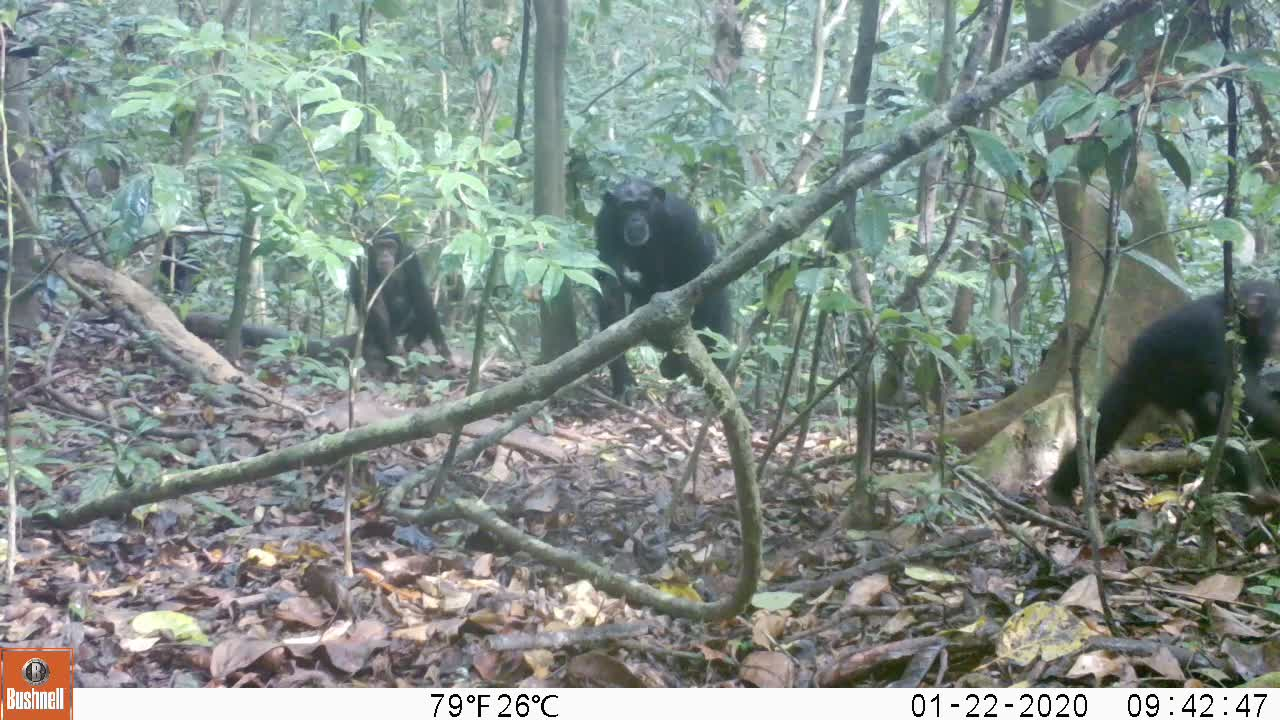
\includegraphics[width=\linewidth]{body/experimental/assets/detection_frames/frame1}
    \end{minipage}
    \begin{minipage}[t]{0.48\textwidth}
        \centering
        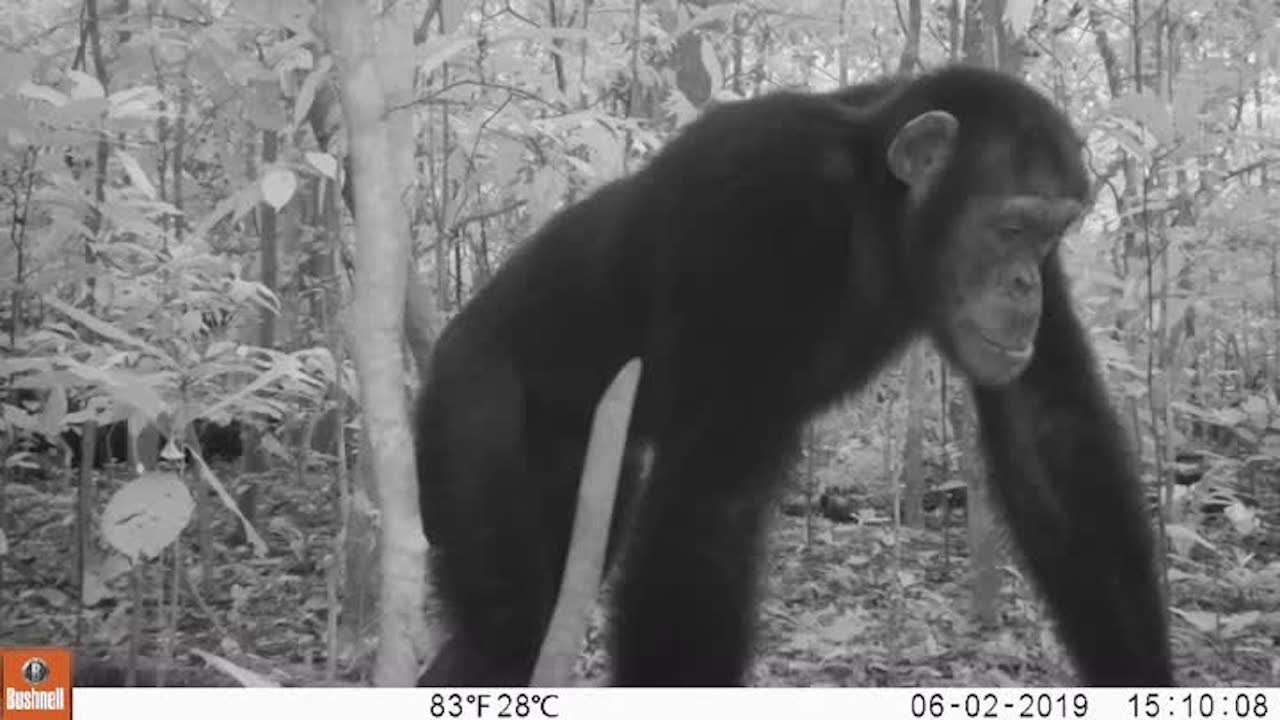
\includegraphics[width=\linewidth]{body/experimental/assets/detection_frames/frame2}
    \end{minipage}

    \begin{minipage}[t]{0.48\textwidth}
        \centering
        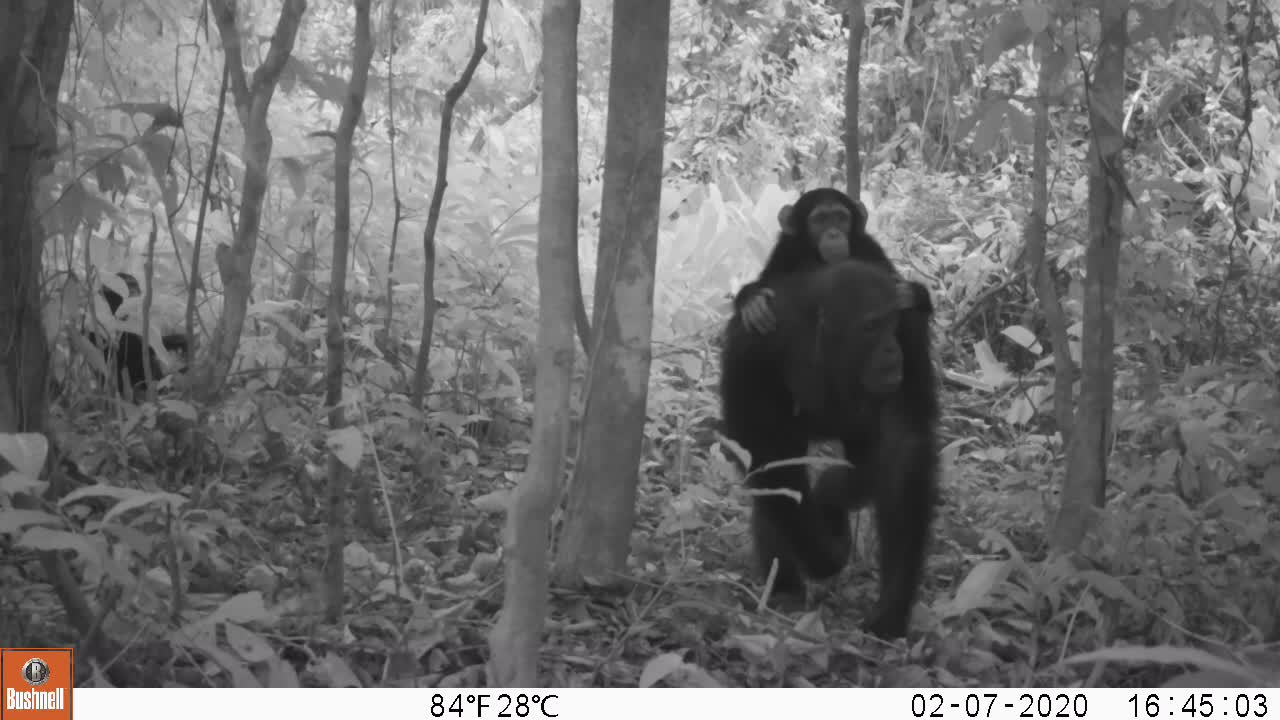
\includegraphics[width=\linewidth]{body/experimental/assets/detection_frames/frame3}
    \end{minipage}
    \begin{minipage}[t]{0.48\textwidth}
        \centering
        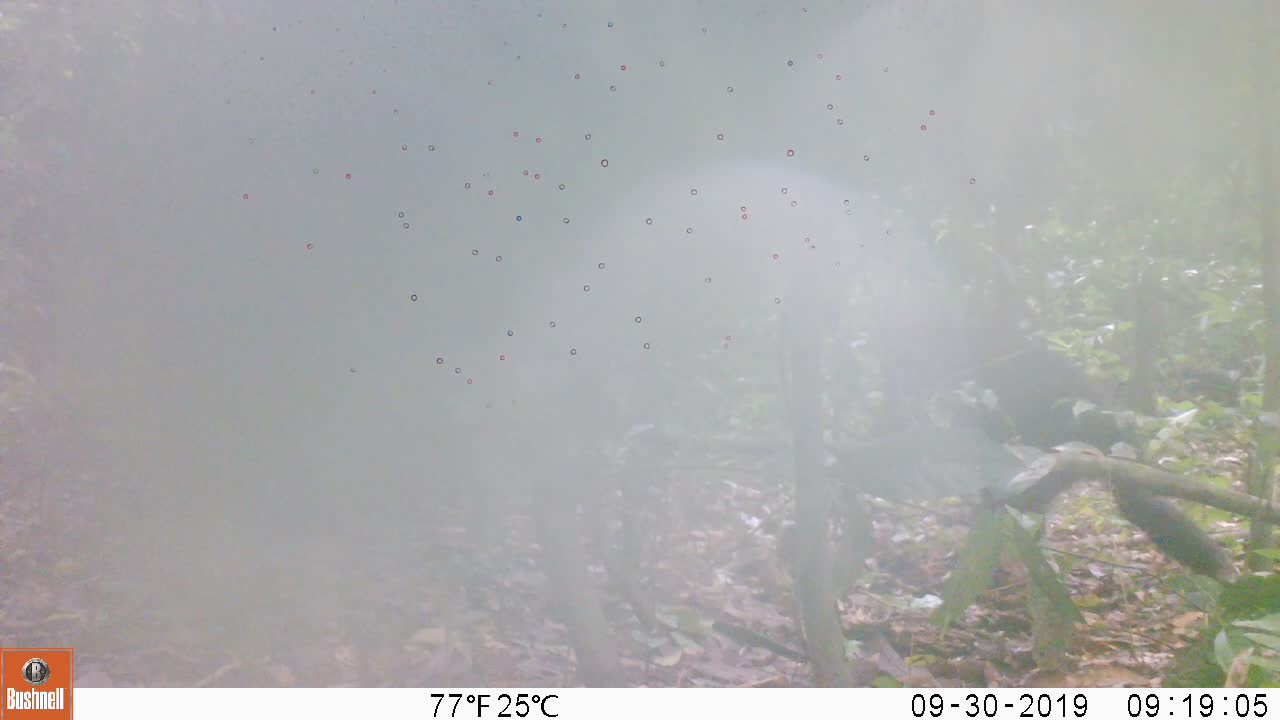
\includegraphics[width=\linewidth]{body/experimental/assets/detection_frames/frame4}
    \end{minipage}

    \begin{minipage}[t]{0.48\textwidth}
        \centering
        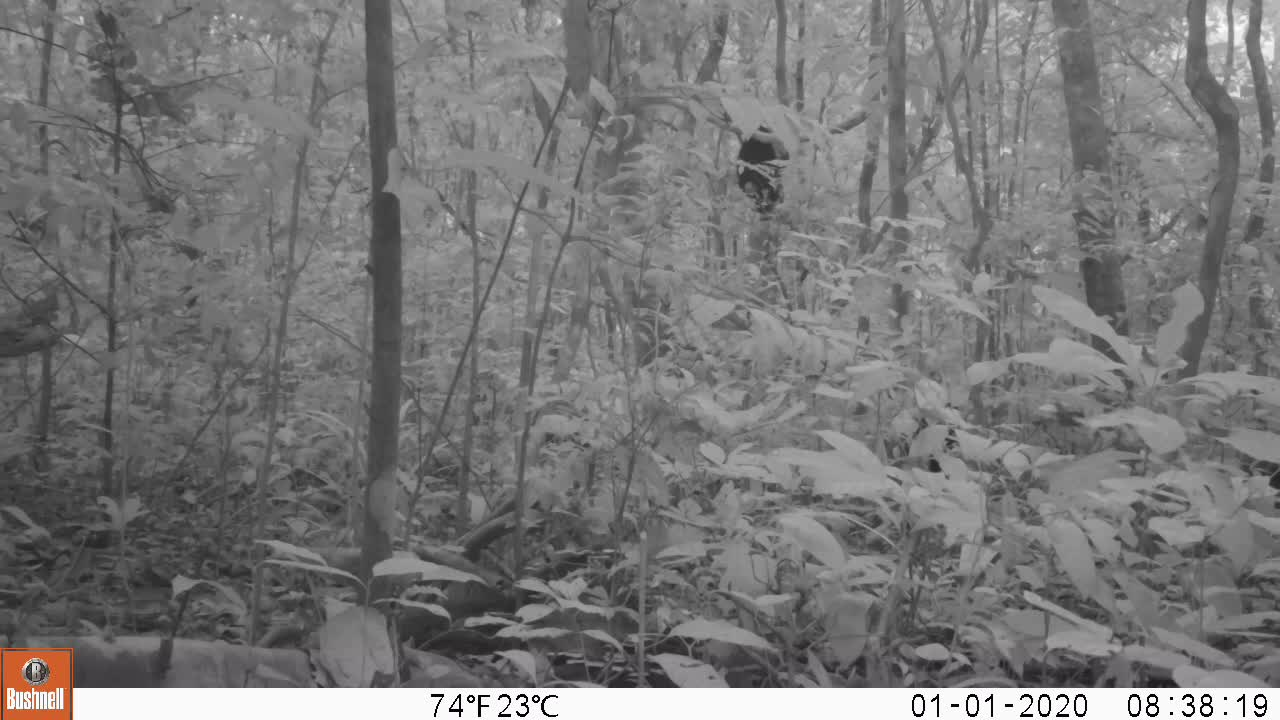
\includegraphics[width=\linewidth]{body/experimental/assets/detection_frames/frame5}
    \end{minipage}
    \begin{minipage}[t]{0.48\textwidth}
        \centering
        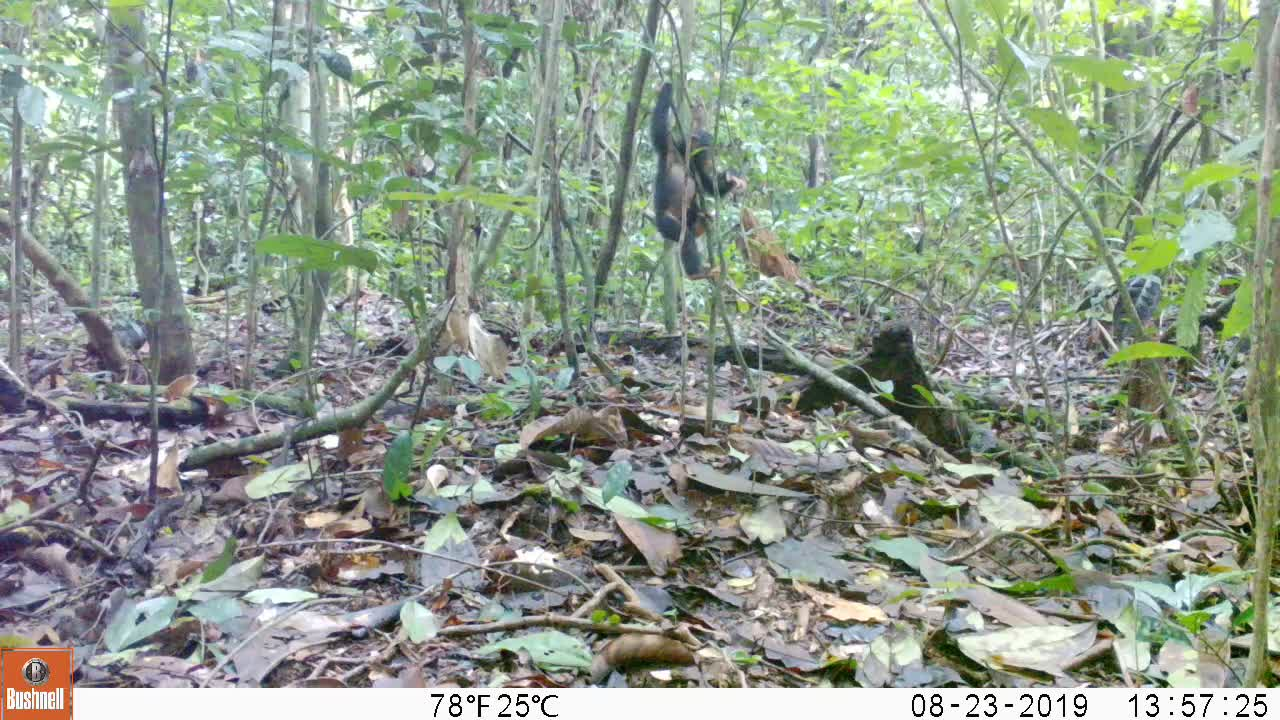
\includegraphics[width=\linewidth]{body/experimental/assets/detection_frames/frame6}
    \end{minipage}

    \begin{minipage}[t]{0.48\textwidth}
        \centering
        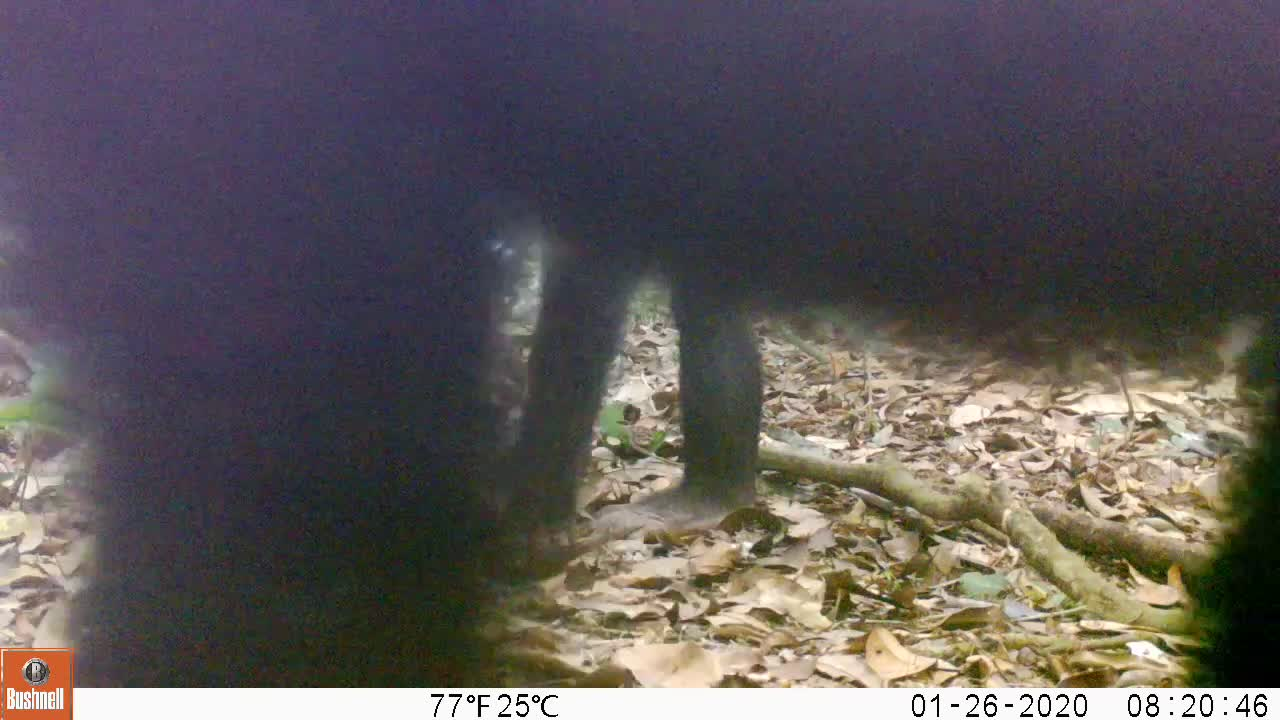
\includegraphics[width=\linewidth]{body/experimental/assets/detection_frames/frame7}
    \end{minipage}
    \begin{minipage}[t]{0.48\textwidth}
        \centering
        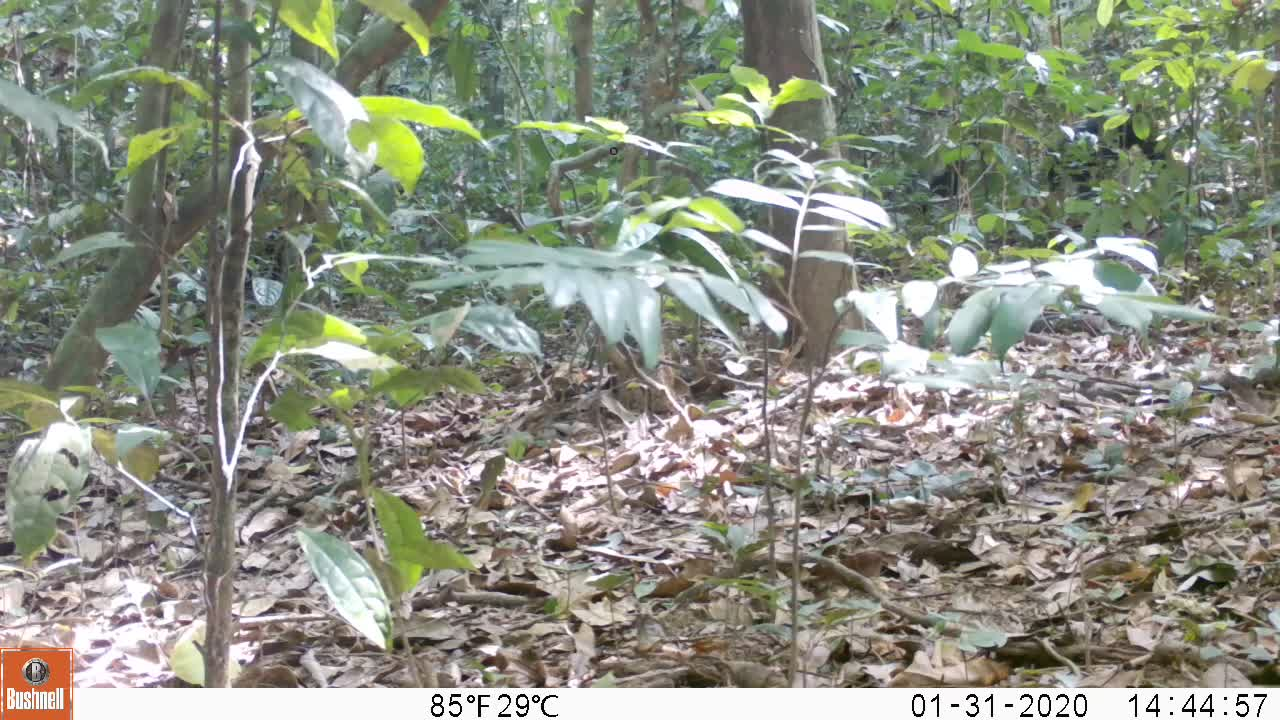
\includegraphics[width=\linewidth]{body/experimental/assets/detection_frames/frame8}
    \end{minipage}
    \caption{Mixed subsample of extracted detection frames capturing chimpanzees\\
    (taken from both the manual and automated sample)}
    \label{fig:detection_frames}
\end{figure}



\begin{figure}[htbp]
    \centering
    \makebox[0.8\textwidth][c]{
        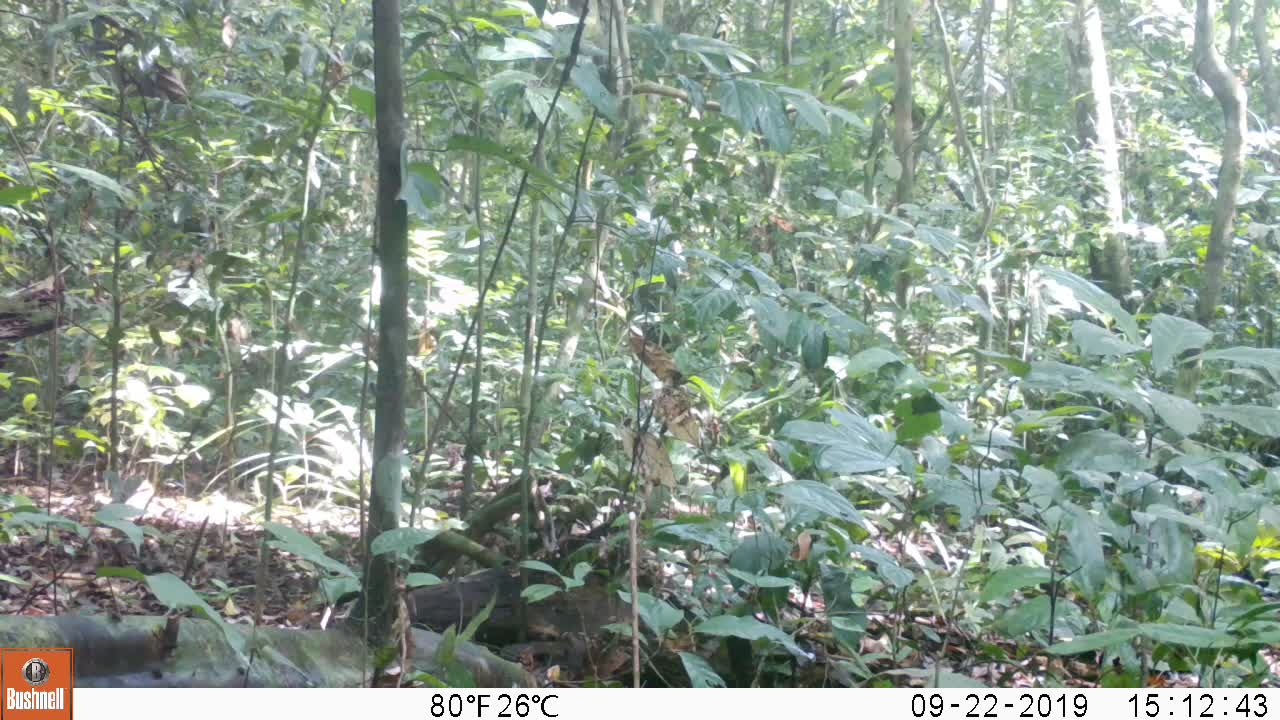
\includegraphics[width=0.8\textwidth]{body/experimental/assets/detection_frames/empty1}
    }\\[1mm]
    \makebox[0.8\textwidth][c]{
        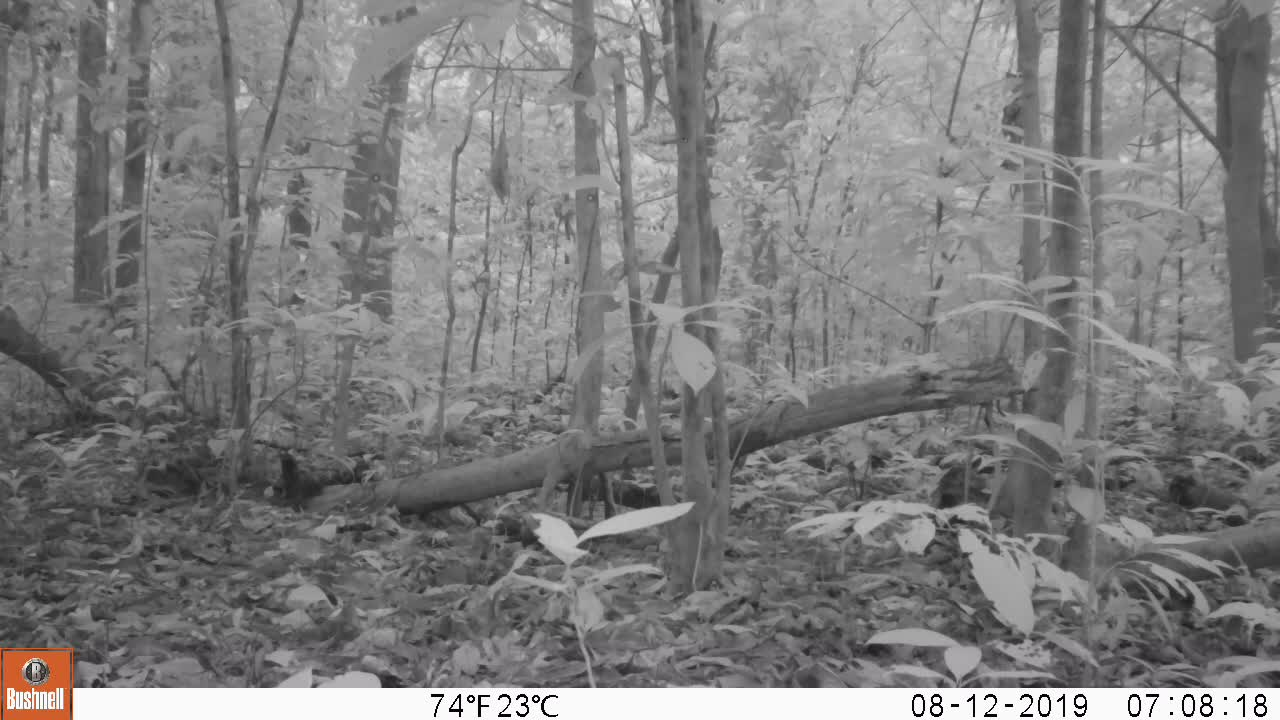
\includegraphics[width=0.8\textwidth]{body/experimental/assets/detection_frames/empty2}
    }
    \makebox[0.8\textwidth][c]{
        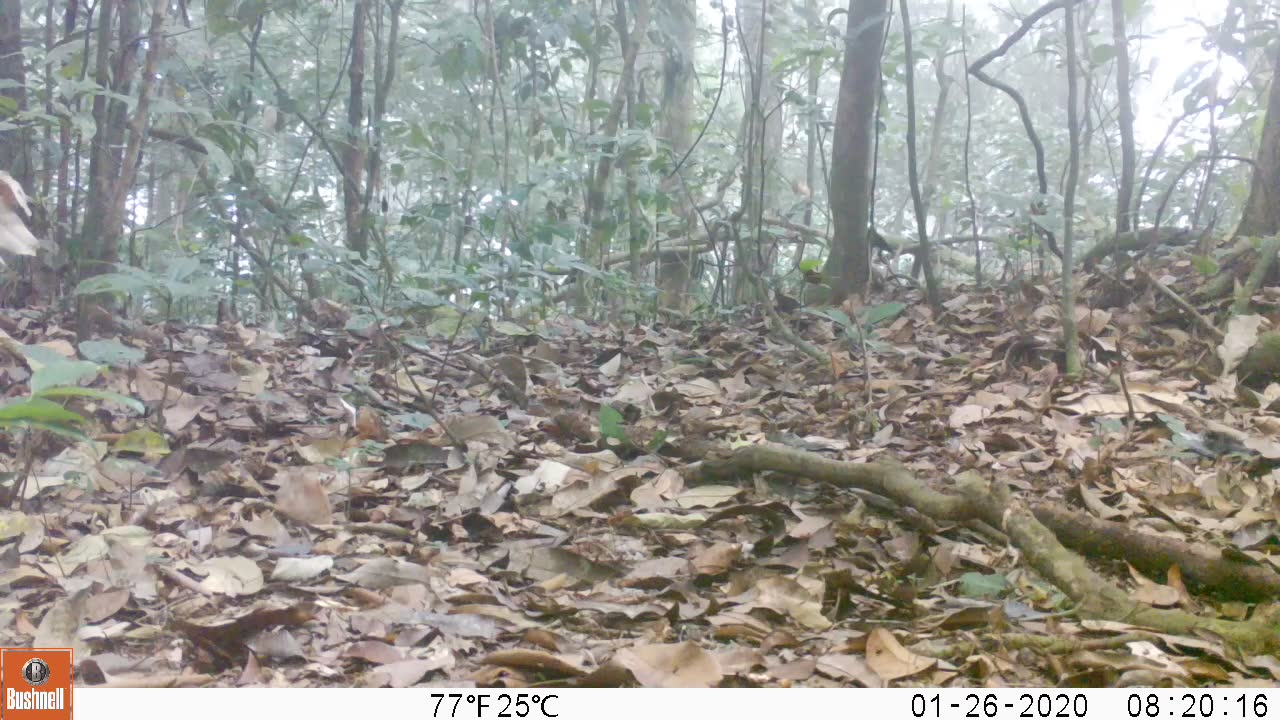
\includegraphics[width=0.8\textwidth]{body/experimental/assets/detection_frames/empty3}
    }
    \caption{Mixed subsample of empty detection frame\\
    (taken exclusively from the automated sample)}
    \label{fig:empty_detection_frames}
\end{figure}